\documentclass[12pt, a4paper]{report}
\usepackage[T1]{fontenc}
\usepackage[utf8]{inputenc}
\usepackage[english]{babel}
\usepackage{frontespizio}
\usepackage[big]{layaureo}
\usepackage{graphicx}
\usepackage{booktabs}
\usepackage{caption}
\captionsetup{tableposition=top,figureposition=bottom,font=small}
\usepackage{tabularx}
\usepackage{subfig}
\usepackage{color}
\usepackage{colortbl}
\definecolor{Gray}{gray}{0.9}
\usepackage{verbatim}
\usepackage{framed}
\definecolor{shadecolor}{gray}{0.97}
\usepackage{biblatex}

\begin{document}
\chapter*{Project 3}
		
The aim of this project is to build a multiclass image classifier based on convolutional neural networks for the provided dataset (ref). 15 categories are present already divided into trainset (1500 images, 100 per category) and test set (2985 images).
	
	
\section{Baseline}
\subsection*{Problem statement}
	
As initial thing we build a first CNN which act as a baseline. Its performance are then compared with the results of some improved CNNs (section 2) and other classifiers based on pretrained CNNs (section 3).
	
\subsection*{Approach}

First of all we  defined the structurs needed to feed the network with our data.\\
Specifically we built a new Dataset class which, every time an image is accessed, loads the image itself in memory and apply a given transformation to it.\\
Then, after having splitted the training dataset into train and validation data, we construcetd two dataloaders which, at each epoch, take care of divide data in batches and give them to the network. The same approach is also used for test data.

After having defined the needed structures we buil a convolutional neural network following the requests, we trained it and finally test it.
	
\subsection*{Implementation choices}

In order to obtain images having size 64x64, we defined a transformation, consisting in an anisotropic rescaling, to apply to each image when loaded.\\
Then, to build the training and the validation dataloaders, we split the given dataset in two parts. The validation dataloader access to the 15\% of the images, equally distributed among the classes, and load them all at once. The traning dataloader access the remaining 85\% of the data, which are loaded in batches of size 32, as required.

After that we've built the network following the given architecture:
	
\begin{table}[h!]
	\centering
	\begin{tabular}{lll}
		\# & Type & Size \\
		\midrule
		1 & Image Input & 64x64x1 images \\
		2 & Convolution & 8 3x3 convolutions with stride 1 \\
		3 & ReLu & \\
		4 & Max Pooling & 2x2 max pooling with stride 2 \\
		5 & Convolution & 16 3x3 convolutions with stride 1 \\
		6 & ReLu & \\
		7 & Max Pooling & 2x2 max pooling with stride 2 \\
		8 & Convolution & 32 3x3 convolutions with stride 1 \\
		9 & ReLu & \\
		10 & Fully Connected & 15 \\
		11 & Softmax & softmax \\
		12 & Classification Output & crossentropyex \\
		\bottomrule
		\label{tab:baseline}
	\end{tabular}
\end{table}
	
Since we've used cross entropy as loss function, and in python this loss already performs softmax, the corresponding layer is not present in the network. So the output of the network are scores and not probabilities.
	
As optimizer we've employed the stochastic gradient descent with learning rate 0.01, momentum 0.9, as set by default.
	
The weights of each layer have been initialized with a gaussian distribution with mean 0 and standard deviation 0.01. The bias of each layer has been set to 0.

Setting the parameters in this way, we were not able to reach a test accuracy of around 30\%. Indeed our network performed as a random classifier, having a test accuracy of less then 7\%. In particular the specified weights were too high for the last two layers using the default learning rate. To reach a statisfactory accuracy, using the required weight initialization, a smaller learning rate was necessary, so we set it to 0.001.

We employed, as a stopping criterion, the early stoppung. We've made this choice because, even if we may not reach the global minimum of the validation loss, we can train for fewer epochs stopping when the validation loss significantly increase.\\
In our specific implementation we evaluate the validation loss every 5 iterations. At each iteration we compare the validation loss with the best one obtained up to that moment. If the current loss is higher then the saved one, we increase a counted. On the other hand, if the current loss is lower then the saved one we update it, save the parameters of the network and set the counter to zero. We stop the training when a certain number of epochs are performed or when the counter reach the value of the patiecnce. In our case we have decided to perform at most $30$ epochs and set the patience to $15$
	
\subsection*{Results}

We performed the training as specified above and plot the evolution of the accuracy and of the loss.

\begin{figure}[h!]
	\centering
	%{\includegraphics[width=.49\textwidth]{img/baseline_accuracy}}
	\label{fig:baselineaccuracy}
	%{\includegraphics[width=.49\textwidth]{img/baseline_loss}}
	\label{fig:baselineloss}
\end{figure}

\section{CNN improvements}
\subsection*{Problem statement}
After having developed a CNN which act as a baseline, we tried to improve the obtained results. In order to do so we applied some transformation to the training data, added some layers and changed some optimizaion parameters. After having found the optimal network we have also build an ensemble of networks.

\subsection*{Description of the approach}
First of all we perform data augmentation. Since the training set is quite small and only contains 1500 images, applying some random transformations on the original data set allows to increase the diversity of the training set itself. In this specific case we apply a random horizontal flip to each image in the training set only, while the validation and the test sets remain the same.

After that we added some layers to the baseline network.\\
Specifically we added a Batch Normalization layer before each reLu layer. In this way the following transformation is applied to the output of the preceding layer:
$$ y = \frac{x - E[x]}{\sqrt{VAR[x]}} * \gamma + \beta$$
The mean $E[x]$ and the standard-deviation $\sqrt{VAR[x]}$ are calculated over the mini-batches and their estimations are then employed during the evaluation phase to normalize the input images. The two parameters $\gamma$ and $\beta$ are vectors of size equal to the input size learned during the training. Thanks to the addition of this layer we avoid divergence of the optimizer due to large changes in the input distribution to each layer. It also reduce dependence on the initialization and acts as a regularizer.\\
We also add a dropout layer before the fully connected one. In this way, during the training phase, some of the outputs of the layer before are randomly set to zero with a given probability. This technique has proven to be effective for regularization and helps in avoinding overfitting.

Then we changed the size of the convolutional filters increasing their support, going from intput to output, to 3x3, 5x5 and 7x7. In order to obtain an output image of the same size of the input one, we added some replicate padding around the image itself. Specifically we set one padding in the first convolutional layer, two in the second and three in the third. In this way the image do not change size going through the network.

Finally we changed some of the optimization parameters.\\
As first thing we introduced weight normalization. Large values of the network weights can lead to unstable performances and can be an indicator of overfitting of the training data set. To avoid this problem we introcuced a regularization term in the objective function which force the network to keep the weight small. In this way the objective function to minimize becomes
$$J(w) = \frac 1 N \sum_{i=1}^n L(f(x_i, w), y_i) + \lambda R(w)$$\\
In addition we introduced a learning rate scheduler which decays the learning rate by a given factor every $n$ epochs.\
As last imporovement we changed the used optimizer switching to Adam optimizer, which is faster than the Stochastic Gradient Descent but is still able to obtain the same performances.

\subsection*{Implementation choices}
In order to augment the training data we defined a new transformation performing both the needed resize and the random horizontal flip with a probability of $0.5$.\\
After having introduced the abouve mentioned additional layers, our improved network had the structure reported in the Table \ref{tab:final}.

\begin{table}[h!]
	\centering
	\begin{tabular}{lll}
		\# & Type & Size \\
		\midrule
		1 & Image Input & 64x64x1 images \\
		2 & Convolution & 8 3x3 convolutions with stride 1 and padding replicate 1 \\
		3 & Batch Normalization & 8 \\
		4 & ReLu & \\
		5 & Max Pooling & 2x2 max pooling with stride 2 \\
		6 & Convolution & 16 5x5 convolutions with stride 1 and padding replcate 2 \\
		7 & Batch Normalization & 16 \\
		8 & ReLu & \\
		9 & Max Pooling & 2x2 max pooling with stride 2 \\
		10 & Convolution & 32 7x7 convolutions with stride 1 and padding replicate 3 \\
		11 & Batch Normalization & 32 \\
		9 & ReLu & \\
		10 & Dropout & p = 0.25 \\
		11 & Fully Connected & 15 \\
		12 & Softmax & softmax \\
		13 & Classification Output & crossentropyex \\
		\bottomrule
		\label{tab:final}
	\end{tabular}
\end{table}

The objective function we aim to minimize was 
$$J(w) = \frac 1 N \sum_{i=1}^n L(f(x_i, w), y_i) + \lambda R(w)$$\\
where $L(f(x_i, w), y_i)$ is the Cross-entropy loss function and the regularization term $R(w)$ is the $L_2$ penalty. In addition we set the $\lambda$ parameter to $0.02$.\\
Concerning the oprimization parameters we set the initial learning rate to $0.001$ and, through the scheduler, it was multiplied by a factor equal to $0.7$ every $3$ epochs. As already said we used Adam as optimizer.\\

\subsection*{Results}

Keeping the training option as for the baseline, whihc is to say performing an early stop setting the patience to $10$ evaluations, we ran the training and plot the evolution of the accuracy and of the loss.

\begin{figure}[h!]
	\centering
	{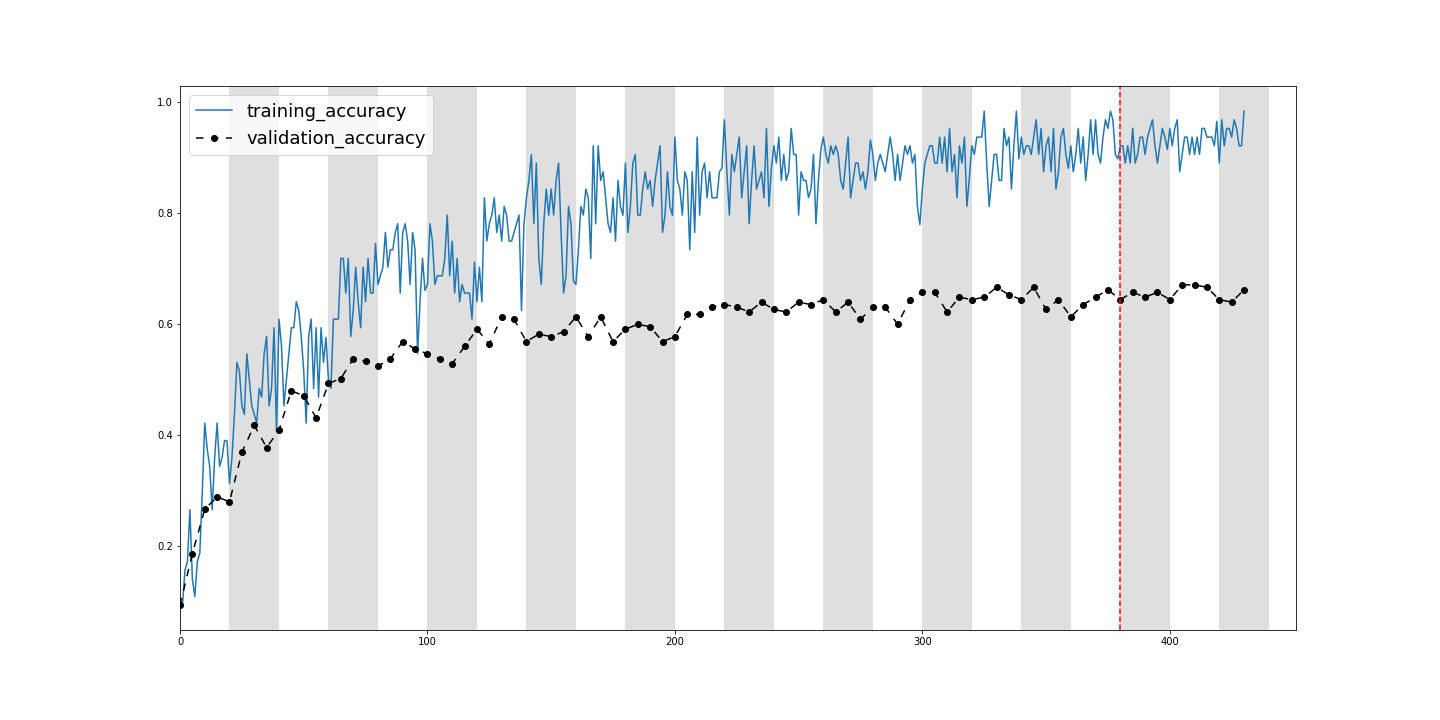
\includegraphics[width=.49\textwidth]{img/final_accuracy}}
	\label{fig:accuracy}
	{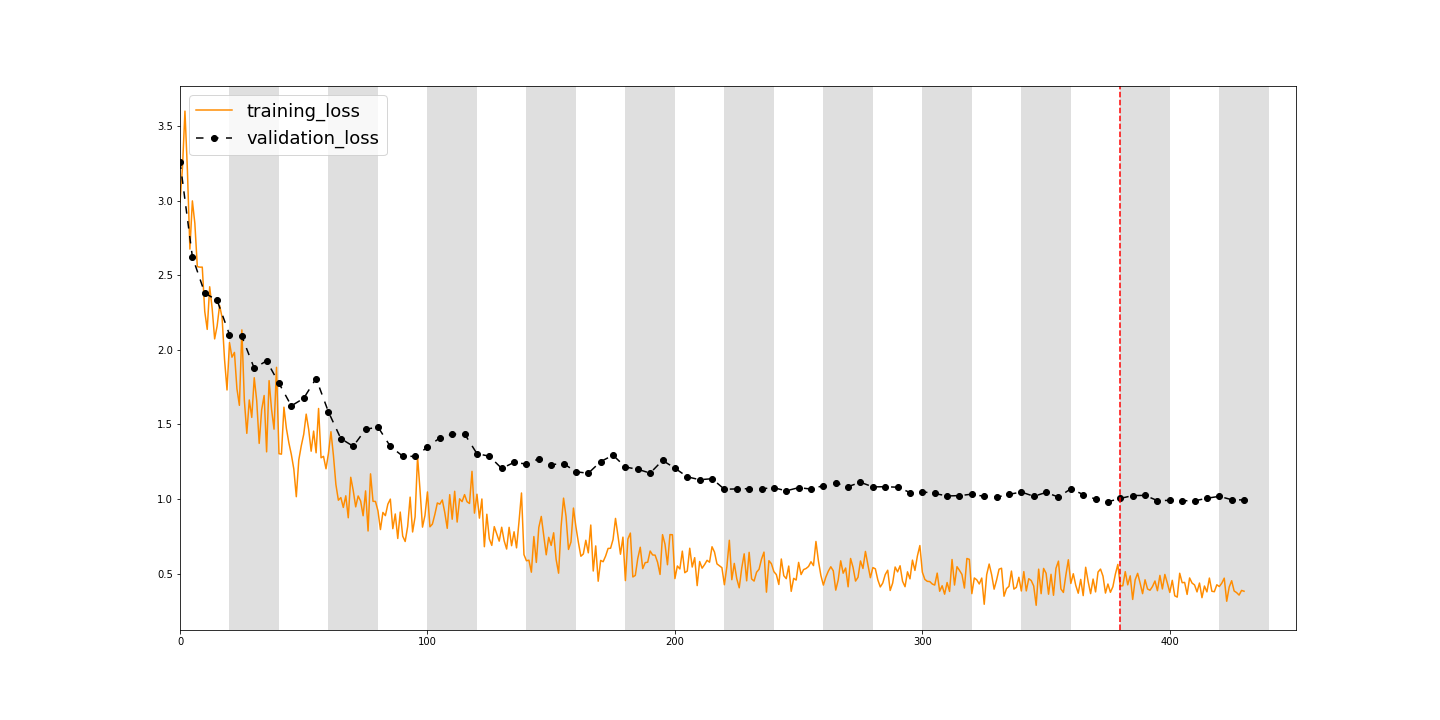
\includegraphics[width=.49\textwidth]{img/final_loss}}
	\label{fig:loss}
\end{figure}

As we can see the training accuracy tends to one, while the validation accuracy is stabilized around the value $0.6$. In a similar way the training loss tends to zero, while the vaidation loss is stabilized around $1$.

Subsequently we test the trained network on the test set and we obtained satisfactory results. Indeed we obtained a test Accuracy of 0.6576214405360133.

We also compute the accuracy matrix which confirms the good performances of the network. Even if we still notice some misclassification expecially among Livingroom and Kitchen and few other classes we are quite satisfied with the obtained result.

\begin{figure}[h!]
	\centering
	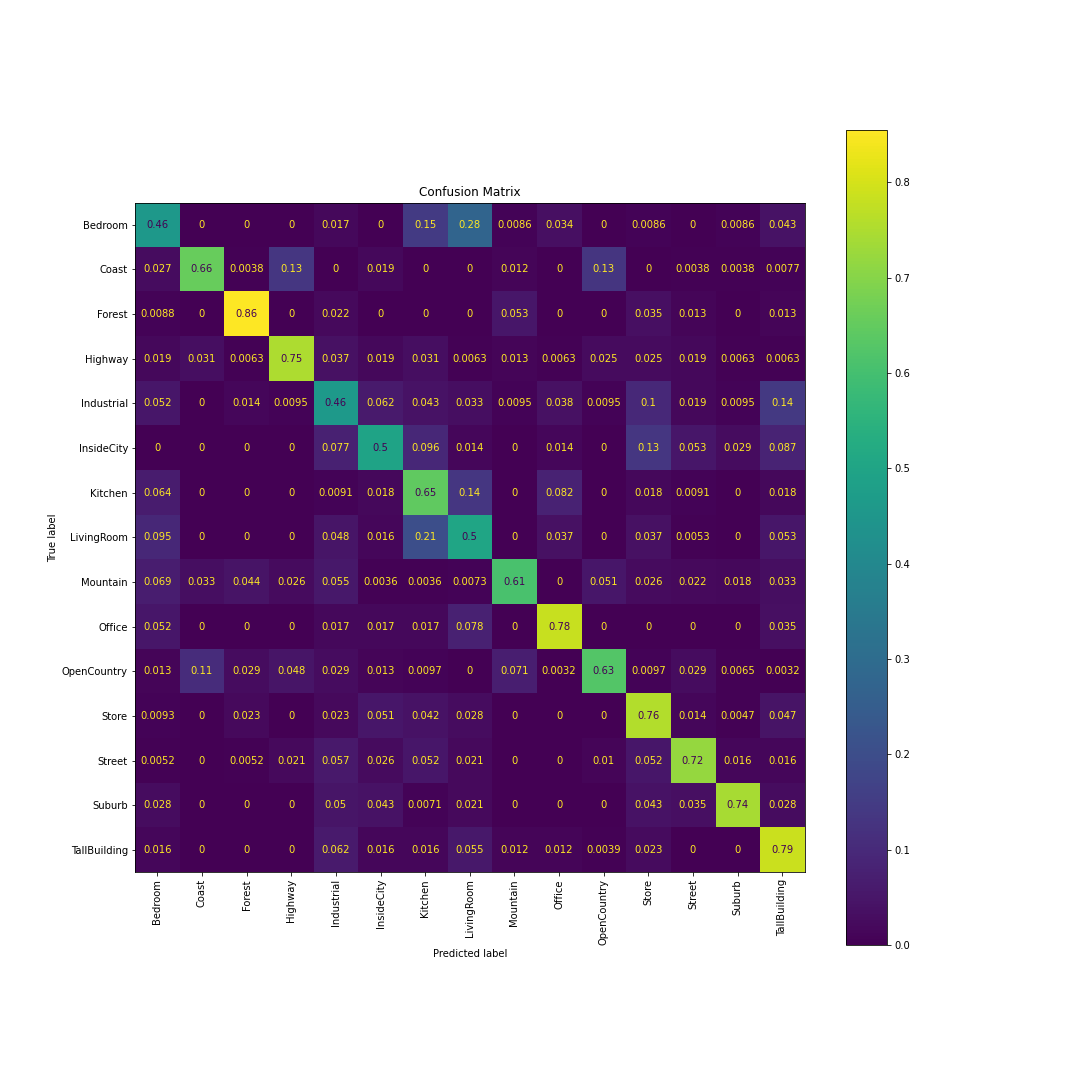
\includegraphics[width=0.9\textwidth]{img/final_cmatrix_norm}
	\label{fig:cmatrix}
\end{figure}

\subsection*{Ensemble of networks}

Our improved convolutional neural network performed good enough but its results were quite unstable. Hence, in order to  reduce the dependence of the CNN on the training data and so reduce the variance of the predictions, we build an esemble of nwtworks, which is to say we build and train several models and combine their predictions together.

Since our dataset is quite small we employed the bootstrap technique. Specifically, after having divided our data into training and validation, we build the training dataloader by sampling with repetition from the selected images. In this way we are able to train the networks on slightly different datasets without reducing the number of used images.

We initialized five instances of neural network having the structure specified above. For each instance we create a different training dataloader using the bootstrap technique which allow us to train them indipendently. After the training phase we test each network on the test set. We apply each network to each image, make a softmax transformation in order to convert the output scores into probabilities. At this point we calculate the average probability of each class computing the arithmetic mean of the output probabilities of the networks. Finally we predict the class having the higher average probability.

Combining the results of independent networks slightly increase our perormances in terms of test accuracy. Nevertheless the main achievements obtainied in this way was the reduced variability of the results. 

\section{Transfer learning}
\end{document}

